% === Begin Label Data ===
% ID: 762
% 难度星级: 
% 标签: 
% 备注: 
% 组卷引用次数: 0
% === End  Label Data ===

\begin{problem}{2026}{G}{上海春考卷}{10}{向量}
在 $\triangle ABC$ 中，$D$、$E$ 在 $BC$ 上，且 $\overrightarrow{BD}=\overrightarrow{DE}=\overrightarrow{EC}$，$|\overrightarrow{AD}|=1$，$\overrightarrow{AD}$ 与 $\overrightarrow{AE}$ 的夹角为 $\dfrac{\pi}{3}$，则 $\overrightarrow{AB}\cdot\overrightarrow{AC}$ 的最大值为 \underline{\hspace{4em}}.
\end{problem}

\begin{answer}
$-\dfrac{39}{32}$
\end{answer}

\begin{solutions}

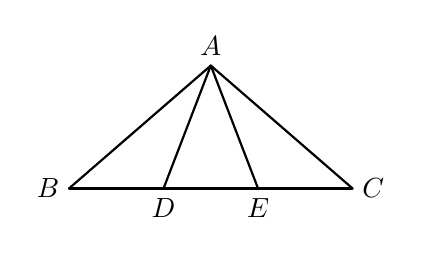
\begin{tikzpicture}[line cap=round,line join=round,scale=0.6]
% points on base BC with D,E trisecting: BD=DE=EC
\coordinate (B) at (0,0);
\coordinate (C) at (6,0);
\coordinate (D) at (2,0);
\coordinate (E) at (4,0);

% apex A (placed above between D and E, like the figure)
\coordinate (A) at (3,2.6);

% segments
\draw[thick] (B) -- (C);
\draw[thick] (A) -- (B);
\draw[thick] (A) -- (C);
\draw[thick] (A) -- (D);
\draw[thick] (A) -- (E);

% labels
\node[left]  at (B) {$B$};
\node[right] at (C) {$C$};
\node[below] at (D) {$D$};
\node[below] at (E) {$E$};
\node[above] at (A) {$A$};

\end{tikzpicture}
 设 $|AE|=t$.  

因为 $\overrightarrow{AB}=\overrightarrow{AD}+\overrightarrow{DB}$，$\overrightarrow{AC}=\overrightarrow{AE}+\overrightarrow{EC}=\overrightarrow{AE}-\overrightarrow{DB}$，且 $\overrightarrow{DB}=\overrightarrow{ED}=\overrightarrow{AD}-\overrightarrow{AE}$，  

所以 $\overrightarrow{AB}\cdot\overrightarrow{AC}=(2\overrightarrow{AD}-\overrightarrow{AE})\cdot(2\overrightarrow{AE}-\overrightarrow{AD})=5\overrightarrow{AD}\cdot\overrightarrow{AE}-2|\overrightarrow{AE}|^{2}-2|\overrightarrow{AD}|^{2}$  

$=5t\cos\dfrac{\pi}{3}-2t^{2}-2=-2t^{2}+\dfrac{5}{2}t-2$.  设 $f(t)=-2t^{2}+\dfrac{5}{2}t-2$，则 $f(t)=-2\left(t-\dfrac{5}{8}\right)^{2}-2+\dfrac{25}{32}$，当 $t=\dfrac{5}{8}$ 时，$\overrightarrow{AB}\cdot\overrightarrow{AC}$ 取最大值 $-\dfrac{39}{32}$.
\end{solutions}